\subsection{Intrinsic dimension from the eigenvalue gap}
  \label{subsec:intrinsic-dimension-from-the-eigenvalue-gap}
  The embedding dimension $d$ is not assumed but is selected by the dominant eigenvalue
  gap $\Delta\lambda_k=\lambda_k-\lambda_{k+1}$.
  Operationally, choose $d$ is chosen as the smallest integer such that
  \begin{equation}
    \Delta\lambda_{d+1} \;>\; \eta\,\lambda_1,
    \label{eq:eigen-gap-criterion}
  \end{equation}
  with a conservative threshold $\eta\sim 0.1$.
  For smooth large-scale configurations, one expects stable low-dimensional embedding
  (often $d=4$ for spacetime-like regimes).

  The spectral criterion used to identify a robust intrinsic dimension is illustrated
  in Fig.~\ref{fig:eigenvalue-gap}.

  \begin{figure}[t]
    \centering
    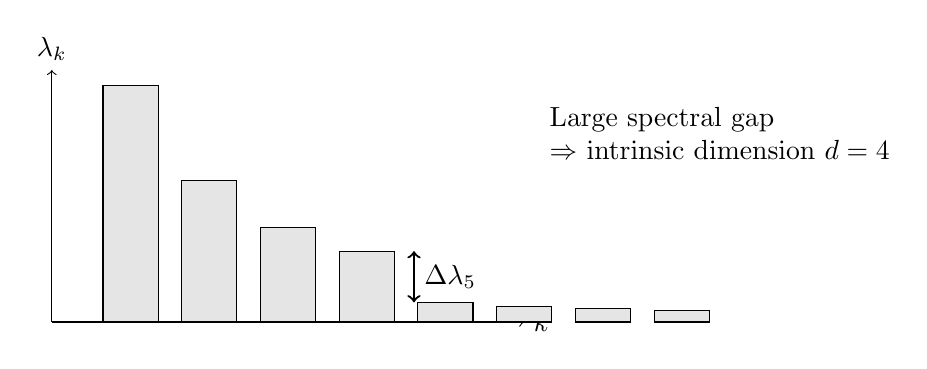
\begin{tikzpicture}[scale=1.0]
        \draw[->] (0,0) -- (6,0) node[right]{$k$};
        \draw[->] (0,0) -- (0,3.2) node[above]{$\lambda_k$};

        % Bars (schematic)
        \foreach \k/\h in {1/3.0,2/1.8,3/1.2,4/0.9,5/0.25,6/0.20,7/0.17,8/0.15} {
          \draw[fill=black!10] (\k-0.35,0) rectangle (\k+0.35,\h);
        }

        % Gap marker
        \draw[<->, thick] (4.6,0.9) -- (4.6,0.25) node[midway,right]{$\Delta\lambda_5$};
        \node[align=left, anchor=west] at (6.2,2.4)
          {Large spectral gap\\$\Rightarrow$ intrinsic dimension $d=4$};
    \end{tikzpicture}
    \caption{\textbf{Schematic eigenvalue spectrum used to select the intrinsic embedding dimension.}
    A clear gap after the first four modes indicates a robust $d=4$ projectable regime.}
    \label{fig:eigenvalue-gap}
  \end{figure}
